\documentclass[10pt, letterpaper]{article}
\usepackage{preamble}
\usetikzlibrary{shapes.multipart}

\begin{document}
\header{CS 6150}{Filemon Mateus}{Homework \#\ 1}{Data Structures}{\today}

\begin{enumerate}[label={\bfseries Q\arabic*.}]
  \item
    \begin{enumerate}
      \item
        Consider the following algorithm:
        \vspace{-5mm}
        \begin{center}
          \begin{minipage}{\linewidth}
            \begin{algorithm}[H]
              \caption{$\textsc{Is-Smaller}(A,x,k)$}\label{alg:is-smaller}
              \begin{algorithmic}[1]
                \Require{A min-heap with $n$ distinct keys in an array $A[1,\ldots,n]$, a value $x$, and an integer $k$.}
                \Ensure{``yes'' if the $k$-th smallest key in the heap is smaller than $x$; ``no'' otherwise.}
                \State $c \gets 0$ \Comment{counts the number of keys $a_c \leq x$; if $c = k$, then we're done!}
                \State $S \gets \varnothing$ \Comment{sets an empty stack for processing suitable keys}
                \State $S.push(1)$ \Comment{commence at the root}
                \While{$S.size() > 0$}
                  \State $i \gets S.pop()$
                  \If{$i \leq A.size()$ \textbf{and} $A[i] \leq x$}
                    \State $c \gets c + 1$
                    \If{$c = k$}
                      \State \Return ``no''
                    \EndIf
                    \State $l \gets 2i$
                    \State $r \gets 2i + 1$
                    \If{$l \leq A.size()$}
                      \State $S.push(l)$
                    \EndIf
                    \If{$r \leq A.size()$}
                      \State $S.push(r)$
                    \EndIf
                  \EndIf
                \EndWhile
                \If{$c < k$}
                  \State \Return ``yes''
                \Else
                  \State \Return ``no''
                \EndIf
              \end{algorithmic}
            \end{algorithm}
          \end{minipage}
        \end{center}

        \autoref{alg:is-smaller} just counts, via iterative \textsc{dfs}, the number of keys
        less or equal to $x$ starting from the root. In the event that $k$ of those are
        exhausted, it returns ``no''; otherwise, it returns ``yes''.

      \item
        In analyzing the runtime of \autoref{alg:is-smaller}, we notice that all lines are
        canonical constant time operations, except the while loop in line $4$, which bears
        the bottleneck of the algorithm. So, in order to show that \autoref{alg:is-smaller}
        runs in $O(k)$, it suffices to show that the while loop in line $4$---representing
        the total number of keys processed by $S$---is linear in $k$. \\

        \begin{claim*}
          For arbitrary inputs $A$, $x$, and $k$, the number of keys processed by $S$ does
          not exceed $2k-1$.
        \end{claim*}

        \begin{proof*}
          The number of keys added to $S$ with value less or equal to $x$ is at most $k$.
          Each key with value greater than $x$ is (by lines $11$ and $12$) a child of a key
          less or equal to $x$. Because every key except the root must have a parent key
          with value smaller or equal to $x$, the number of keys with value greater than $x$
          must be at most $2(k-1)-(k-1)$ since $k-1$ of the $2(k-1)$ child keys have values
          smaller or equal to $x$. So, in the worst case, $S$ processes $k$ keys smaller or
          equal to $x$ and $k-1$ greater than $x$, which amounts to $2k-1$ keys in total!
        \end{proof*}

        With this established, $T(n) = O(2k - 1) + O(1) = O(k)$, as desired!
    \end{enumerate}

  \item
    \begin{enumerate}
      \item
        We proceed with the following strategy: we augment $T$ by transforming it into an order
        statistic tree and supplement its nodes with one additional field, call it $size$. This
        new field, for a given node, say $v$, will store the size of the subtree rooted in $v$,
        which in more practical terms amounts to the number of descendants of $v$ plus one (see
        \autoref{fig:bst-size} for details). With this strategy in mind, we wish to maintain
        the following invariance over $size$: $v.size = v.left.size + v.right.size + 1$.

        \begin{minipage}{\linewidth}
          \begin{figure}[H]
            \centering
            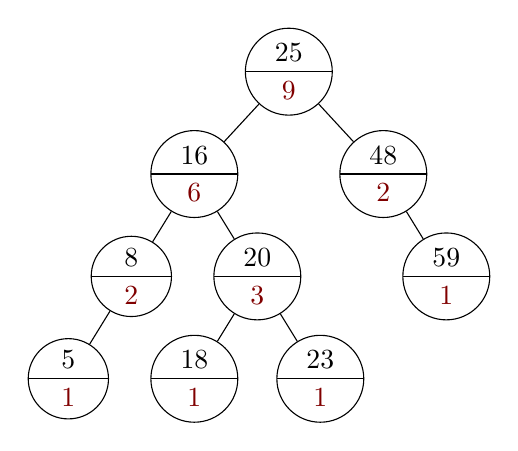
\begin{tikzpicture}[
              level 1/.style={level distance=13mm,sibling distance=24mm},
              level 2/.style={level distance=13mm,sibling distance=16mm},
              level 3/.style={level distance=13mm,sibling distance=16mm},
              level 4/.style={level distance=13mm,sibling distance=16mm},
              every node/.style={minimum width=1em, draw, circle split},
              every lower node part/.style={red!50!black}
            ]
              \node {$25$ \nodepart{lower} $9$}
              child {node {$16$ \nodepart{lower} $6$}
                child {node {$8$ \nodepart{lower} $2$}
                  child {node {$5$ \nodepart{lower} $1$}}
                  child [missing]
                }
                child {node {$20$ \nodepart{lower} $3$}
                  child {node {$18$ \nodepart{lower} $1$}}
                  child {node {$23$ \nodepart{lower} $1$}}
                }
              }
              child {node {$48$ \nodepart{lower} $2$}
                child [missing]
                child {node {$59$ \nodepart{lower} $1$}}
              };
            \end{tikzpicture}
            \caption{
              Order Statistic Tree constructed from $T$. Note each node is augmented with an
              additional field (in red) denoting its $size$.
            }
            \label{fig:bst-size}
          \end{figure}
        \end{minipage}

      \item
        Now, consider the following algorithm, which given a value $x$, computes its $rank$:
        \vspace{-5mm}
        \begin{center}
          \begin{minipage}{\linewidth}
            \begin{algorithm}[H]
              \caption{$\textsc{Rank}(T,x)$}\label{alg:rank}
              \begin{algorithmic}[1]
                \Require{An augmented and balanced order statistic tree and a value $x$.}
                \Ensure{The position of $x$ (one-indexed!) in the linear sorted list of keys of the tree.}
                \State $r \gets 0$ \Comment{the rank of $x$ in $T$}
                \State $v \gets T.root$
                \While{$v \neq \textsc{nil}$}
                  \If{$v.key \leq x$}
                    \If{$v.left \neq \textsc{nil}$}
                    \State $r \gets r + v.left.size + 1$ \Comment{count the \# of elements less than $v$ + $v$ itself}
                    \Else
                      \State $r \gets r + 1$ \Comment{if there isn't a left, just count $v$}
                    \EndIf
                    \If{$v.key = x$}
                      \State \Return{$r$}
                    \EndIf
                    \State $v \gets v.right$ \Comment{explore the right sub-tree}
                  \Else
                    \State $v \gets v.left$ \Comment{explore the left sub-tree}
                  \EndIf
                \EndWhile
                \State \Return{$r+1$} \Comment{plus one to account for key $x$ not in the tree}
              \end{algorithmic}
            \end{algorithm}
          \end{minipage}
        \end{center}

        Suppose $T$ is balanced and augmented. Then at every iteration of the while loop in line $3$,
        \autoref{alg:rank} reduces the problem space by half by carefully choosing to explore either
        the left sub-tree or the right sub-tree. This means \autoref{alg:rank} only traverses a single
        path in $T$ to find the $rank$ of $x$. But any path's length in $T$ is bounded by $T$'s height---$\log_{}n$.
        So, in the worst case, the length of the path traced by \autoref{alg:rank} is exactly $\log_{}n$,
        which incurs an $O(\log_{}n)$ in its runtime.

      \item
        Let $v$ be an arbitrary node in $T$. Then, since the $size$ attribute of $v$ only depends on
        information on $v.left$ and $v.right$, according to the \textbf{Main Theorem}, we can maintain
        the values of $size$ in all nodes of $T$ during $insertion$ and $deletion$ without affecting the
        desired $O(\log_{}n)$ time performance of these operations. Moreover, since $size$ only equips
        $T$ with additional information, the time performance of $search$ operations remains unchanged.
    \end{enumerate}

  \item
    \begin{enumerate}
      \item
        Consider the following algorithm on a balanced binary search tree $T$ whose keys are distinct:
        \vspace{-5mm}
        \begin{center}
          \begin{minipage}{\linewidth}
            \begin{algorithm}[H]
              \caption{$\textsc{Range-Query}(v,x_l,x_r)$}\label{alg:range-query}
              \begin{algorithmic}[1]
                \Require{A node $v$ in $T$ and two real numbers $x_l$ and $x_r$, denoting a range.}
                \Ensure{All keys $x$ stored in $T$ such that $x_l \leq x \leq x_r$.}
                % \State $u \gets$ \Call{\textsc{min-ge}}{$T, x_l$} \Comment{minimum node with key greater or equal to $x_l$}
                % \State $v \gets$ \Call{\textsc{max-se}}{$T, x_r$} \Comment{maximum node with key smaller or equal to $x_r$}
                % \State $w \gets$ \Call{\textsc{lca}}{$T, x_l, x_r$} \Comment{lowest common ancestor between $x_l$ and $x_r$}
                % \State $S \gets \varnothing$ \Comment{empty stack for iterative in-order traversal}
                % \State $R \gets \varnothing$ \Comment{solution: array of keys of $T$ in range $[x_l, x_r]$}
                % \State
                % \While{$S.size() > 0$ \textbf{or} $(w \neq \textsc{nil}$ \textbf{and} $w.key \in [u.key, v.key])$}
                %   \If{$w \neq \textsc{nil}$ \textbf{and} $w.key \in [u.key, v.key]$}
                %     \State $S.push(w)$
                %     \State $w \gets w.left$
                %   \Else
                %     \State $w \gets S.pop()$
                %     \State $R.push(w.key)$
                %     \State $w \gets w.right$
                %   \EndIf
                % \EndWhile
                % \State \Return{$R$}
                % \State
                % \Procedure{\textsc{min-ge}}{$T, x_l$}
                %   \State $u \gets \textsc{nil}$
                %   \State $n \gets T.root$
                %   \While{$n \neq \textsc{nil}$}
                %     \If{$n.key \geq x_l$}
                %       \State $u \gets n$
                %       \State $n \gets n.left$
                %     \Else
                %       \State $n \gets n.right$
                %     \EndIf
                %   \EndWhile
                %   \State \Return{$u$}
                % \EndProcedure
                % \State
                % \Procedure{\textsc{max-se}}{$T, x_r$}
                %   \State $u \gets \textsc{nil}$
                %   \State $n \gets T.root$
                %   \While{$n \neq \textsc{nil}$}
                %     \If{$n.key \leq x_r$}
                %       \State $u \gets n$
                %       \State $n \gets n.right$
                %     \Else
                %       \State $n \gets n.left$
                %     \EndIf
                %   \EndWhile
                %   \State \Return{$u$}
                % \EndProcedure
                % \Procedure{\textsc{lca}}{$T, x_l, x_r$}
                %   \State $u \gets T.root$
                %   \While{$(u \neq \textsc{nil})$ \textbf{and} $(u.key < x_l$ \textbf{or} $u.key > x_r)$}
                %     \If{$u.key > x_r$}
                %       \State $u \gets u.left$
                %     \EndIf
                %     \If{$u.key < x_l$}
                %       \State $u \gets u.right$
                %     \EndIf
                %   \EndWhile
                %   \State \Return{$u$}
                % \EndProcedure
                \If{$v \neq \textsc{nil}$}
                  \If{$x_l \leq v.key$}
                    \State \Call{\textsc{Range-Query}}{$v.left, x_l, x_r$} \Comment{search left for potential candidates}
                  \EndIf
                  \If{$x_l \leq v.key \leq x_r$}
                    \State \Call{\textsc{Print}}{$v.key$}
                  \EndIf
                  \If{$v.key \leq x_r$}
                    \State \Call{\textsc{Range-Query}}{$v.right, x_l, x_r$} \Comment{search right for potential candidates}
                  \EndIf
                \EndIf
              \end{algorithmic}
            \end{algorithm}
          \end{minipage}
        \end{center}

      \item
        Let $k$ be number of keys of $T$ who fall in the range $[x_l, x_r]$. Then, in either execution
        path, \autoref{alg:range-query} always terminates by reporting exactly $k$ values of $T$ which
        means the \textsc{Print} statement in line $6$ is called exactly $k$ times---one for each value
        in the range. Assume this operation is constant, since we have $k$ of those we get an $O(k)$ cost
        for reporting/printing the values in the range. Added to this cost are the two recursive calls
        in line $3$ and $9$ that search (through only one path!) down to the height of $T$.  Now, since
        $T$ is balanced the two recursive calls incur both an $O(\log n)$ time cost each. \\

        So, putting all together, if we let $T(n)$ represent the total time taken for \autoref{alg:range-query}
        to report $k$ of $n$ keys of $T$ in the range $[x_l, x_r]$ then $T(n) = O(k) + O(\log n) + O(\log n) =
        O(k + \log n)$. This last equality follows from the fact that $k$ may very well exhaust all nodes 
        in the tree, in which case $k = n \gg \log n$.
    \end{enumerate}

  \item
    \begin{enumerate}
      \item
        We augment $T$ as follows: for every entry node $v$ in $T$, we supplement $v$ with one additional field,
        call it $sum$. This new field will store the cumulative sum of all the values descendants of $v$ as well
        as the value of $v$ itself (see \autoref{fig:bst-sum} for details). With this augmentation, we wish to 
        maintain the following invariance over $sum$: $v.sum = v.left.sum + v.right.sum + v.key$.

        \begin{minipage}{\linewidth}
          \begin{figure}[H]
            \centering
            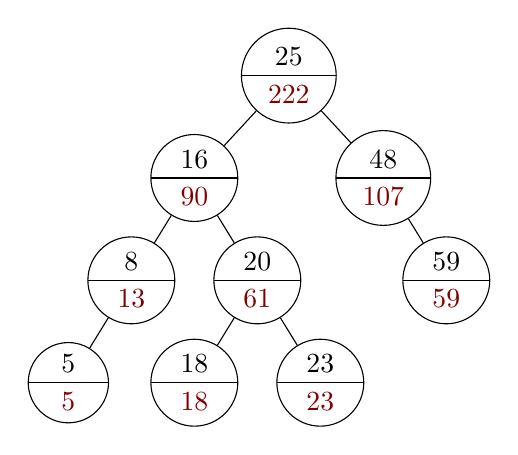
\begin{tikzpicture}[
              level 1/.style={level distance=13mm,sibling distance=24mm},
              level 2/.style={level distance=13mm,sibling distance=16mm},
              level 3/.style={level distance=13mm,sibling distance=16mm},
              level 4/.style={level distance=13mm,sibling distance=16mm},
              every node/.style={minimum width=1em, draw, circle split},
              every lower node part/.style={red!50!black}
            ]
              \node {$25$ \nodepart{lower} $222$}
              child {node {$16$ \nodepart{lower} $90$}
                child {node {$8$ \nodepart{lower} $13$}
                  child {node {$5$ \nodepart{lower} $5$}}
                  child [missing]
                }
                child {node {$20$ \nodepart{lower} $61$}
                  child {node {$18$ \nodepart{lower} $18$}}
                  child {node {$23$ \nodepart{lower} $23$}}
                }
              }
              child {node {$48$ \nodepart{lower} $107$}
                child [missing]
                child {node {$59$ \nodepart{lower} $59$}}
              };
            \end{tikzpicture}
            \caption{
              Augmented and Balanced Binary Search Tree constructed from $T$. Note each node $v$ is augmented with
              an additional field (in red) representing its $sum$.
            }
            \label{fig:bst-sum}
          \end{figure}
        \end{minipage}

      \item
        Now consider the following algorithm, which given a range $[x_l, x_r]$, returns the sum of all
        keys of $T$ in that range:
        \vspace{-5mm}
        \begin{center}
          \begin{minipage}{\linewidth}
            \begin{algorithm}[H]
              \caption{$\textsc{Range-Sum}(T,x_l,x_r)$}\label{alg:range-sum}
              \begin{algorithmic}[1]
                \Require{An augmented and balanced binary search tree and two real numbers $x_l$ and $x_r$, denoting a range.}
                \Ensure{The sum of all keys of $T$ in the range $[x_l, x_r]$.}
                \State $S_L \gets 0$ \Comment{sum of all keys $< x_l$}
                \State $v \gets T.root$
                \While{$v \neq \textsc{nil}$}
                  \If{$v.key < x_l$}
                    \If{$v.left \neq \textsc{nil}$}
                      \State $S_L \gets S_L + v.left.sum + v.key$
                    \Else
                      \State $S_L \gets S_L + v.key$
                    \EndIf
                    \State $v \gets v.right$
                  \Else
                    \State $v \gets v.left$
                  \EndIf
                \EndWhile
                \State
                \State $S_R \gets 0$ \Comment{sum of all keys $\leq x_r$}
                \State $v \gets T.root$
                \While{$v \neq \textsc{nil}$}
                  \If{$v.key \leq x_r$}
                    \If{$v.left \neq \textsc{nil}$}
                      \State $S_R \gets S_R + v.left.sum + v.key$
                    \Else
                      \State $S_R \gets S_R + v.key$
                    \EndIf
                    \State $v \gets v.right$
                  \Else
                    \State $v \gets v.left$
                  \EndIf
                \EndWhile
                \State
                \State \Return{$S_R - S_L$} \Comment{sum of all keys in $[x_l, x_r]$}
              \end{algorithmic}
            \end{algorithm}
          \end{minipage}
        \end{center}

        In analyzing the runtime of \autoref{alg:range-sum}, we notice that there are two almost identical pieces
        in its structure (namely, lines $1$--$14$ and lines $16$--$29$). In both of these pieces, we start at the
        root of the tree and make a decision to either walk left or right. We stop until a leaf node is reached.
        So, the paths traced by these lines ($1$--$14$ and $16$--$29$) cannot exceed the height of $T$---$\log n$.
        This is because every time we make a decision to walk left or right, we are effectively narrowing the search
        space by half. But since the search space initially starts with $n$ (the number of nodes in the tree), we are
        restricted to at most $\log n$ steps in that walk until $n$ gets reduced to $1$, in which case, we are in the presence
        of a leaf node. So, lines $1$--$14$ and $16$--$29$ both incur an $O(\log n)$ cost each, and a direct consequence
        of this is that the total running time of \autoref{alg:range-sum} is:
        \[
          T(n) = O(\log n) + O(\log n) + O(1) = O(\log n)
        \]
        The last equality follows from the fact that $O(1)$ is also $O(\log n)$, so we get $3O(\log n) = O(\log n)$
        as required!

      \item
        Let $v$ be an arbritrary node in $T$. Then, since---per $sum$ invariance in part a---the $sum$ attribute of $v$ only
        depends on information on $v$, $v.left$, and $v.right$, according to the \textbf{Main Theorem}, we can maintain
        the values of $sum$ in all nodes of $T$ during $insertion$ and $deletion$ without affecting the desired $O(\log n)$
        time performance of these operations. Moreover, since $sum$ only equips $T$ with additional information, the time
        performance of $search$ operations remains unchanged.

    \end{enumerate}
\end{enumerate}
\end{document}
